% Página
\section{Custódia das Chaves de Criptografia}

No exemplo apresentado, Alice é a usuária Custodiante e Bob é o usuário que terá as suas chaves custodiadas. Assim, todas as chaves do Bob devem ser compartilhadas com a Custodiante Alice.

\subsection{Custodiando}

Bob irá custodiar as suas duas chaves, Chave Privada(KPrBob.pem) e Chave de Dados(DEKBob.bin), com a custodiante Alice.

\begin{figure}[H]
	\centering
	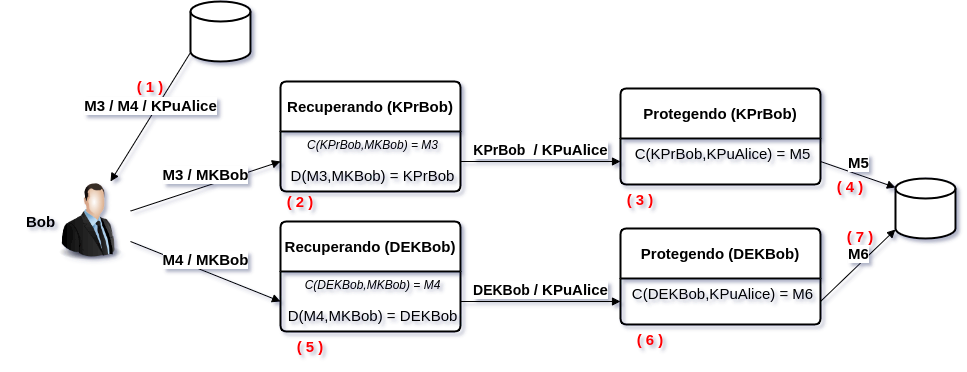
\includegraphics[scale=0.55]{custodiando.png}
	\caption{Processos de Custódia das Chaves do Bob}
	\label{fig:custodiando}
\end{figure}

\begin{enumerate}
	\item Bob recupera os Textos Cifrados M3 e M4 e a Chave Pública da Alice (KPuAlice.pem) do servidor;
	\item Bob descriptografa o Texto Cifrado M3 com sua Chave Mestra (MKBob.hex) e o IV associado para obter sua Chave Privada (KPrBob);
	\begin{tcolorbox}[width=\textwidth]
		{\scriptsize
			\begin{verbatim}
			$ openssl enc -d -aes-256-cbc -K "$(cat MKBob.hex)" -iv "$(cat M3.iv)" \
			  -in M3.bin -out KPrBob.pem
			\end{verbatim}
		}
	\end{tcolorbox}
	\item Bob protege a sua Chave Privada (KPrBob.pem) para a custodiante Alice, gerando o Texto Cifrado M5. O envelope CMS usa criptografia híbrida: cifra o conteúdo e encapsula a chave de conteúdo para o certificado da Alice (Alice.cert.pem).
	\begin{tcolorbox}[width=\textwidth]
		{\scriptsize
			\begin{verbatim}
			$ openssl cms -encrypt -binary -in KPrBob.pem -out M5.pem -outform PEM \
			  -recip Alice.cert.pem -aes256
			\end{verbatim}
		}
	\end{tcolorbox}
	\item Bob envia o Texto Cifrado M5 para o Servidor;
	\item Bob descriptografa o Texto Cifrado M4 com sua Chave Mestra (MKBob.hex) e o IV associado para obter sua Chave de Dados (DEKBob.bin);
	\begin{tcolorbox}[width=\textwidth]
		{\scriptsize
			\begin{verbatim}
			$ openssl enc -d -aes-256-cbc -K "$(cat MKBob.hex)" -iv "$(cat M4.iv)" \
			  -in M4.bin -out DEKBob.bin
			\end{verbatim}
		}
	\end{tcolorbox}
	\item Bob criptografa sua Chave de Dados (DEKBob.bin) com a Chave Pública da Alice (KPuAlice.pem), gerando o Texto Cifrado M6.bin;
	\begin{tcolorbox}[width=\textwidth]
		{\scriptsize
			\begin{verbatim}
			$ openssl pkeyutl -encrypt -inkey KPuAlice.pem -pubin -in DEKBob.bin -out M6.bin \
			  -pkeyopt rsa_padding_mode:oaep -pkeyopt rsa_oaep_md:sha256
			\end{verbatim}
		}
	\end{tcolorbox}	
	\item Bob envia o Texto Cifrado M6 para o Servidor;
\end{enumerate}

\pagebreak
